\documentclass[11pt,a4paper]{article}
\usepackage[utf8]{inputenc}
\usepackage[spanish]{babel}
\usepackage{amsmath}
\usepackage{amsfonts}
\usepackage{amssymb}
\usepackage{makeidx}
\usepackage{graphicx}
\usepackage{lmodern}
\usepackage{kpfonts}
\usepackage{parskip}
\usepackage[left=2cm,right=2cm,top=2cm,bottom=2cm]{geometry}
\author{Miguel Angel Xamie Diaz Fuentes}
\begin{document}
\begin{center}
\begin{LARGE}
\textbf{INGENIERÍA MECATRÓNICA}\\
\end{LARGE}
{\large Sistemas Eletrónicos De Interfaz}\\
\begin{figure}[hbtp]
\centering

\includegraphics[scale=0.80]{UPZMG_Mecatr_nica.png}
\end{figure} 
\begin{center}
\begin{LARGE}
EV-2-8- CALCULAR LOS PARAMETROS DE CIRCUITOS DE ACTIVACIÓN DE TRANSISTORES DE POTENCIA
\end{LARGE}
\end{center}

\begin{Large}
\textbf{Alumno}
\\\textit{Miguel Angel Xamie Diaz Fuentes}
\textbf{\\Maestro}
\\\textit{Morán Garabito Carlos Enrique}
\textbf{\\Fecha de Entrega}
\\\textit{29/10/2019}
\textbf{\\Grupo}
\\\textit{4-B}\\
\textbf{Período Cuatrimestral}\\
\textit{2019-Septiembre-Diciembre}
\\
\end{Large}

\end{center}

\footnote{Universidad Politécnica De La Zona Metropolitana De Guadalajara} 

\newpage

\section{Transistores de Potencia}

El funcionamiento y utilización de los transistores de potencia es idéntico al de los transistores normales, teniendo como características especiales las altas tensiones e intensidades que tienen que soportar y, por tanto, las altas potencias a disipar.

Existen tres tipos de transistores de potencia:
\begin{itemize}
\item Bipolar.
\item Unipolar o FET (Transistor de Efecto de Campo).
\item IGBT.
\end{itemize}

\begin{figure}[hbtp]
\centering
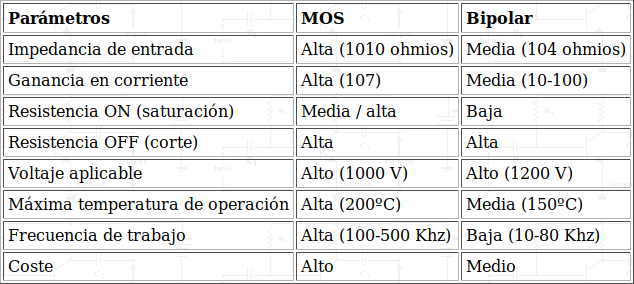
\includegraphics[scale=0.80]{1.png}
\end{figure}
El IGBT ofrece a los usuarios las ventajas de entrada MOS, más la capacidad de carga en corriente de los transistores bipolares: 
\begin{itemize}
\item Trabaja con tensión.
\item Tiempos de conmutación bajos.
\item Disipación mucho mayor (como los bipolares)
\end{itemize}

Nos interesa que el transistor se parezca, lo más posible, a un elemento ideal: 

\begin{itemize}

\item Pequeñas fugas.
\item Alta potencia.
\item Bajos tiempos de respuesta (ton , toff), para conseguir una alta frecuencia de funcionamiento.
\item Alta concentración de intensidad por unidad de superficie del semiconductor.
\item Que el efecto avalancha se produzca a un valor elevado (VCE máxima elevada).
\item Que no se produzcan puntos calientes (grandes di/dt).

\end{itemize}

Una limitación importante de todos los dispositivos de potencia y concretamente de los transistores bipolares, es que el paso de bloqueo a conducción y viceversa no se hace instantáneamente, sino que siempre hay un retardo (ton , toff). Las causas fundamentales de estos retardos son las capacidades asociadas a las uniones colector - base y base - emisor y los tiempos de difusión y recombinación de los portadores. 
\footnote{Universidad Politécnica De La Zona Metropolitana De Guadalajara} 

\newpage

\section{Funcionamiento}

La diferencia entre un transistor bipolar y un transistor unipolar o FET es el modo de actuación sobre el terminal de control. En el transistor bipolar hay que inyectar una corriente de base para regular la corriente de colector, mientras que en el FET el control se hace mediante la aplicación de una tensión entre puerta y fuente. Esta diferencia vienen determinada por la estructura interna de ambos dispositivos, que son substancialmente distintas.

Es una característica común, sin embargo, el hecho de que la potencia que consume el terminal de control (base o puerta) es siempre más pequeña que la potencia manejada en los otros dos terminales.

En resumen, destacamos tres cosas fundamentales: 

\begin{itemize}

\item En un transistor bipolar IB controla la magnitud de IC.
\item En un FET, la tensión VGS controla la corriente ID.
\item En ambos casos, con una potencia pequeña puede controlarse otra bastante mayor. 
\end{itemize}

\section{Modos de Trabajo}
Existen cuatro condiciones de polarización posibles. Dependiendo del sentido o signo de los voltajes de polarización en cada una de las uniones del transistor pueden ser:

\begin{figure}[hbtp]
\centering
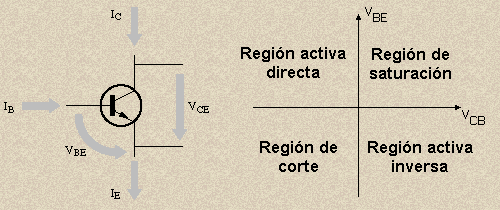
\includegraphics[scale=0.80]{2.png}
\end{figure}

\begin{itemize}

\item Región activa directa: Corresponde a una polarización directa de la unión emisor - base y a una polarización inversa de la unión colector - base. Esta es la región de operación normal del transistor para amplificación.
\item Región activa inversa: Corresponde a una polarización inversa de la unión emisor - base y a una polarización directa de la unión colector - base. Esta región es usada raramente.
\item Región de corte: Corresponde a una polarización inversa de ambas uniones. La operación en ésta región corresponde a aplicaciones de conmutación en el modo apagado, pues el transistor actúa como un interruptor abierto (IC 0).
\item Región de saturación: Corresponde a una polarización directa de ambas uniones. La operación en esta región corresponde a aplicaciones de conmutación en el modo encendido, pues el transistor actúa como un interruptor cerrado (VCE 0). 


\end{itemize}

\footnote{Universidad Politécnica De La Zona Metropolitana De Guadalajara} 

\newpage

\section{Ejercicio de Ejemplo}

\begin{figure}[hbtp]
\centering
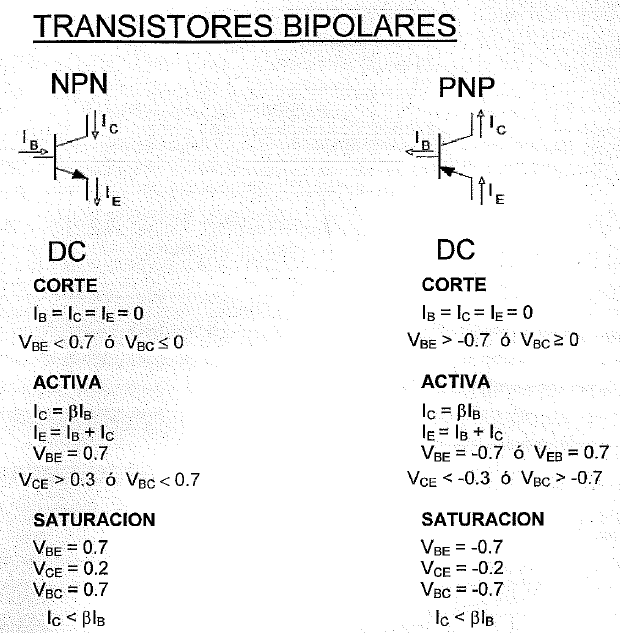
\includegraphics[scale=0.60]{3.png}
\end{figure}

\subsection{Problema 1} 

Diseñe un circuito de excitación de la base de un BJT, con la configuración de la figura, que tenga un pico de 3 A durante la puesta en conducción y mantenga una corriente de base de 0,4 A mientras el transistor está activado. La tensión vi es un pulso de 0 a 50 V con un ciclo de trabajo del 50 por ciento, y la frecuencia de conmutación es de 100kHz. Suponga que vBE es de 1 V cuando el transistor está conduciendo. 

\footnote{Universidad Politécnica De La Zona Metropolitana De Guadalajara} 

\newpage

\begin{figure}[hbtp]
\centering
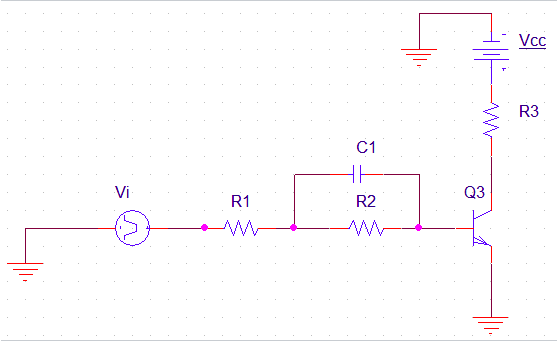
\includegraphics[scale=0.60]{4.png}
\end{figure}
\textit{Circuito de Excitación para un Transistor Bipolar}

\textbf{Solución}

El valor de R1 viene determinado por la necesidad del pico inicial de corriente. Despejando R1 en la siguiente fórmula:

\begin{Huge}
$ R_1 = \frac{V_i - V_{BDE}}{I_{B1}} $

$ R_1 = \frac{50 - 1}{3} $

$ R_1 = 16\Omega $
\end{Huge}

 La corriente de base en conduccion en régimen permanente determina el valor de R2: 
 
 \begin{Huge}
$ R_1 = \frac{V_i - V_{BDE}}{I_{B2}} - R_1 = 106\Omega $
 \end{Huge}
 
El valor de C se calcula a partir de la constante de tiempo necesaria. Para un ciclo de trabajo del 50 por ciento a 100 kHz, el transistor conduce durante 5us. Haciendo que el tiempo de conducción del transistor sea cinco veces la constante de tiempo, t=1us:

\begin{Huge}
$ \tau = R_e * C = \frac{R_1 * R_2}{R_1 + R_2} * C = (13,9)C = 1us   $

$ C = 0,072 uF
 $
\end{Huge}

\footnote{Universidad Politécnica De La Zona Metropolitana De Guadalajara} 

\newpage


\subsection{Problema 2}

El circuito de la figura, tiene Vcc = 90 V, L = 200 mH, R= 20 ohm, t1= 10 ms y T= 100 ms. Determine: a) La corriente de pico y la energía de pico acumulada en la bobina. b) La potencia media absorvida por la resistencia y c) la potencia media y de pico suministrada por la fuente.
 
\begin{figure}[hbtp]
\centering
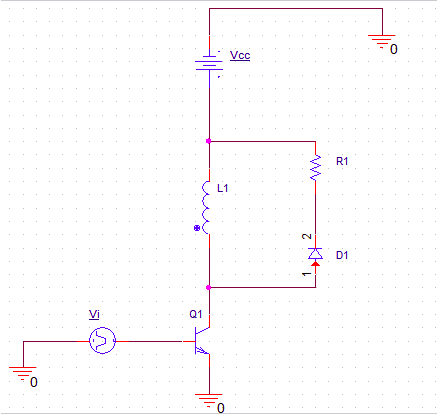
\includegraphics[scale=0.60]{5.png}
\end{figure}
\textit{Circuito de alimentación de una bobina y transferencia de energía almacenada a una resistencia}

\textbf{Solución}

 Para empezar calcularemos la corriente de la bobina cuando el transistor está activado:
 
\begin{Huge}
$ i_L = \frac{Vcc}{L} = \frac{90}{0,2} = 470tA \longrightarrow 0 \prec t \prec 10ms$
\end{Huge}

La corriente de pico de la bobina y la energia almacenada es: 

\begin{Huge}
$ i_L(t1) = 450(0,01) = 4,5A $

$ W_L = \frac{1}{2} Li^2 (t_1)= \frac{1}{2}(0,2)(4,5)^2 = 4,5A$
\end{Huge}

b) La constante del tiempo para la corriente cuando el interruptor está abierto es L/R = 200 mH/20 ohm = 10 ms. El interruptor está abierto durante 90 ms, que es igual a 10 constantes de tiempo, por lo que prácticamente toda la energía almacenada en la bobina se transfiere a la resistencia: 

\begin{huge}
$ W_R = W_L = 2,025J $

\end{huge} 

La potencia media absorbida por la resistencia se determina a partir de la siguiente ecuación: 

\footnote{Universidad Politécnica De La Zona Metropolitana De Guadalajara} 

\newpage

 \begin{Huge}
  $ P_R = \frac{W_R}{T} = \frac{2,025}{0,1} = 20,25W $
  \end{Huge} 

c) La corriente de la fuente es igual a la corriente de la bobina cuando el interruptor está cerrado y es cero cuando el interruptor está abierto. La potencia instantánea entregada por la fuente es: 

\begin{figure}[hbtp]
\centering
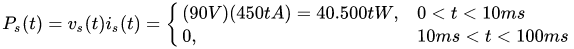
\includegraphics[scale=0.60]{7.png}
\end{figure}

con un valor máximo de 405 W en t = 10 ms. La potencia media suministrada por la fuente puede determinarse a partir de la siguiente ecuación: 

\begin{figure}[hbtp]
\centering
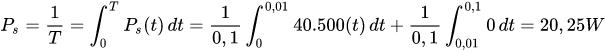
\includegraphics[scale=0.60]{6.png}
\end{figure}

La media de la forma de onda triangular de corriente de la fuente durante un periodo es: 

\begin{Huge}
$ I_8 = \frac{1}{2} \frac{(0,01s)(4,5A)}{0,1s} =  0,025A $
\end{Huge}

y la potencia media de la fuente por lo tanto es: 

\begin{Huge}
$ P_8 = V_ccI_8 = (90V)(0,225A) = 20,25W $
\end{Huge}

Si nos damos cuenta, la potencia absorbida por la resistencia es igual a la suministrada por la fuente: 

\begin{Huge}
$ P_S = P_R = 20,25W $
\end{Huge}

\footnote{Universidad Politécnica De La Zona Metropolitana De Guadalajara} 

\newpage


\bibliography{Referencia}
\begin{thebibliography}{X}

\bibitem{Baz} \textsc{M.GAUDRY.} \textit{Rectificadores, tiristores y triacs.} Ed.Paraninfo, Madrid.

\bibitem{Baz} \textsc{M.J.FISHER.} \textit{Power electronics.} 
PWS-KENT.


\bibitem{Baz} \textsc{H. RASHID MUHAMMAD.} \textit{Power electronics, circuits, devices and applications.} Prentice Hall.

\bibitem{Baz} \textsc{HAMDI HABIB-ALLAH, ANTONIO GALLO TORRES, J.D. AGUILAR PEÑA E.U.} \textit{Elementos semiconductores de pontecia: transistores, diodos.} Politecnica de Jaen, departamento de electrónica.

\bibitem{Baz} \textsc{J.D. AGUILAR PEÑA.} \textit{Apuntes de la asignatira de electrónica industrial.} Impartidas en la E.U. Politecnica de Jaén.


\end{thebibliography}

\bibliographystyle{plain}

\footnote{Universidad Politécnica De La Zona Metropolitana De Guadalajara} 
















































\end{document}